\chapter{Related work}
In this chapter we survey the studies which focus on problem of irradiance estimation using sky images. The usage of ground-based cameras for studying effect of clouds on irradiation has a long history, as early as 1977 when Borkowski et al.\cite{Borkowski1977} developed the first whole-sky camera system for investigating effects of clouds on middle ultraviolet global radiation. In this study, the degree of solar obstruction and cloud coverage were determined visually from the images. Later in 1998, Jeff Sabburg and Joe wong\cite{Sabburg1998} developed and evalued the first automated, ground-based, sun-centered sky camera system for cloud assessment. However, since the purpose of study was the clouds effect on UVB\footnote{Ultraviolet B} radiation they only considered a small area around the sun for cloud and sun ostruction detection which is of paramount importance for this rays. They use a threshold-based approch on gray scale pixel intensities for cloud detection. They also use solar radiation measurements in a image processing algorithm to reduce reflections from the sun on the camera system being mistaken for cloud in the images.

\section{CAPACITATI}
This work uses sets of two sensequative images  taken by GoPro Hero2 camera(one with normal exposure and the other one under-exposed) to extract RGB, HSV components. Then by identify several threshold, they segment four zone type in each image: sun, blue sky, thin clouds and thick clouds. Finally, a regressor used to estimate direct irradiation (DNI) based on the number of pixels of different zone types in the images. One sample of segmentaion is shown in figure\ref{fig:capatitati}

\begin{figure}[h]
\caption{Three different zones identified in an image (sun, cloud, sky)}
\label{fig:capatitati}
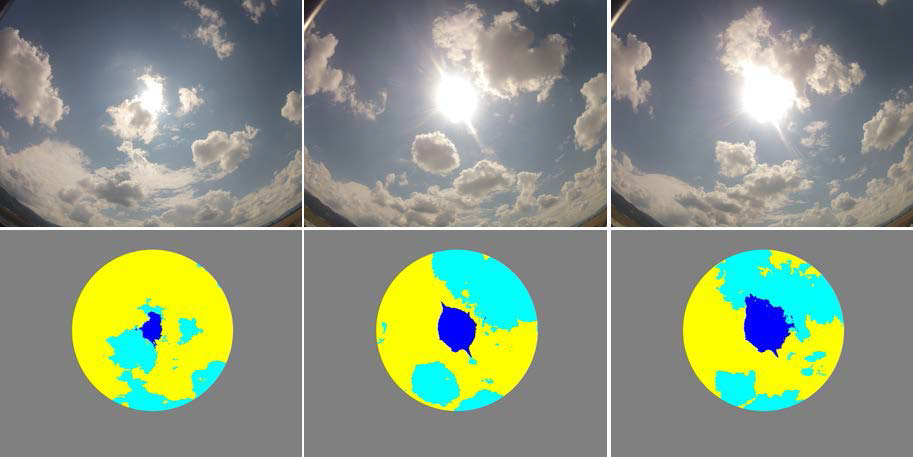
\includegraphics[scale=.5]{capatitati}
\centering
\end{figure} 

\section{T. Schmidt work}
This\cite{tSchmidt15} is the most recent and most relevant work on retrieving irradiation using sky imager pictures.
